\section{Exterior sewing and finite bridge moments}\label{sec:sewing}

Everything here uses pure sides (lattice cuts normal to the \(n_j\)), and the length of a path between cuts counts visited triangle centers. The marked-polygon bound controls two-link events. We first construct exterior connectors, then recover their costs by averaging the cuts. These operations will turn the two-mark estimate into a second length moment.

\begin{proposition}[Confined crossings]\label{prop:corridors}
The following statements hold with constants depending only on the fixed relative tolerances and pure normals.

\begin{itemize}

\item 

Starting at a midpoint with inward normal \(n\), one can travel in that half-plane to a pure terminal line at distance \(s\) from the source whose outward normal \(m\) differs from \(n\) by at most \(60^\circ\), staying before the terminal line until crossing at the end. For any fixed positive relative tolerance, and all sufficiently large admissible \(s\) with a threshold depending only on that tolerance, the travel can be confined within that tolerance around the straight segment in direction \(m\), with mass \(\gtrsim s^{-1/4}\). Also the unrestricted mass in this two-cut domain is \(O(s^{-1/4})\).

\item 

From one specified midpoint to another on the same pure boundary at distance \(l>0\), one can use half-plane arches of diameter \(O(l)\) with mass \(\gtrsim l^{-5/4}\); even without confinement the mass is \(O(l^{-5/4})\).

\end{itemize}
The boundary-to-boundary mass is also decreasing as the terminal port moves away from the source along one straight side of a convex pure-sided truncation, whenever the compared adjacent ports remain on that side.
\end{proposition}
\begin{proof}

For the first assertion, the upper bound is the convex diameter bound (one may truncate by pure convex cuts). For the lower bound with a turn, choose a small fixed \(a>0\) in terms of the requested confinement tolerance. Exit first through the side normal to \(m\) in the centered triangle of size \(s_1\), averaged over admissible \(s_1\in[as,2as]\). The deep-exit estimate \eqref{eq:deep-triangle-exit} retains mass \(\gtrsim s^{-1/4}\) at depth at least a smaller fixed multiple of \(s\) from the base. Then make a bridge along \(m\) to the terminal, confined within a tolerance small even compared with this initial depth, so it stays inside the initial half-plane. This costs \(\gtrsim s^{-1/4}\) more. Joint mass for two choices of the first level splits at both transversal renewals into the triangle exit, the difference bridge and the final bridge, thus averaging \(O(s^{-3/4})\). Cauchy--Schwarz gives mass \(\gtrsim (s^{-1/2})^2/s^{-3/4}=s^{-1/4}\). Without a turn just use the narrow-channel bound.

For the second assertion about confinement, half-plane monotonicity via an artificial arc works also in a convex pure-sided truncation: from \(a<P<Q\) on the same straight side, with \(P,Q\) adjacent, the arc input from \(a\to Q\) directed back to \(P\) can only continue to an exit between \(a,P\) with resulting phase \(z^{-1}\); from \(a\to P\) via the arc to \(Q\), the remaining chord from \(Q\) has \(|W|\le\pi\), and the first two turns cancel. Here we follow the orientation of the earlier adjacent-cap argument, \(z=e^{i\beta\pi}\). Thus after multiplication by \(z\) all outgoing imaginary coefficients are nonnegative just as there. Now in a large centered half-hexagon of scale a fixed multiple of \(l\), the loss from full half-plane arches to ends at distances in \([l,2l]\) is small compared with their total mass of order \(l^{-1/4}\), by the diameter bound. Apply monotonicity inside the truncation.

\end{proof}

\subsection{Two exterior sewing estimates}

Choose a triangular lattice vertex as origin and take the pure-support domains \(D=D(0;\mathbf b)\) of \eqref{eq:pure-support-domain}, with \(|b_j-R|\le\varepsilon R\) for a fixed sufficiently small \(0<\varepsilon\le1/20\). These are convex hexagons. Their minimum side length is then of order \(R\), and Section~\ref{sec:hexagon-completion} supplies the uniform nesting and central-occupancy estimates for every such domain, including independent bounded row roundings.

Use a random nested family \(D_h\) indexed by \(h\) in a window of size \(cR\), \(c>0\) small. Move each nominal support outward at speed 1 from a regular arrangement plus a perturbation \(c' R f(V_i+A_i h/R)\), with \(c'>0\) small, \(f\) a unit-period triangular zigzag of absolute slope 1, \(V_i\) uniform modulo 1, \(A_i\) uniform on \([-1,1]\), independently. Given \(r<s\) in that window, conditional on the phases at \(r\) the nominal supports at \(s\) are independent with densities at most \(C/(s-r)\), since slopes' parameters remain independent and the zigzag has boundedly many monotone branches over the allowed range.

For each facet choose a fixed nondecreasing rounding map to its admissible row levels, depending only on that facet's nominal support and with uniformly bounded error; floor, ceiling, or nearest-level rounding with a fixed tie rule will do. Use the same map at every \(h\). Each nominal support has derivative at least \(1-c'>0\) wherever differentiable, so rounding preserves nesting. It also preserves independence between facets conditional on their inner phases. If its error is at most \(K d_0\), an atom of the rounded support is the image of an interval of length at most \(2K d_0\). Thus the conditional density bound becomes an atom bound \(C\min(1,Kd_0/(s-r))\), sufficient for all the averages below. Boundary gaps are \(O(1+s-r)\) and at least \(c_0(s-r)-O(1)\). The particular monotone rounding here constructs a nested family; the estimates for an individual domain allow every rounding satisfying the displayed support bounds.

Use complete chords in \(D_h\) with ordered boundary ends \(p,q\) binned by dyadic separation \(l\asymp |p-q|\) (of at least constant order) and by the two values \(t_i\) of one plus distance to nearest corner capped at order \(l\), also to within dyadic factors. Orientations do not affect any of our bounds. We describe two sewing estimates for a chord event of mass \(E_h\) in such a bin. Its contents such as marked vertices may be constrained arbitrarily as a deterministic event given \(h,D_h\).

\begin{proposition}[Exterior sewing]\label{prop:exterior-sewing}
For the nested family, endpoint bin and deterministic chord event just specified, the following estimates hold. The average \(\overline E\) includes the level and the support randomness, and the constants are uniform in the event and the admissible levels.
\begin{enumerate}

\item 

If it requires the use of two fixed internal links, the average satisfies
\[
 \overline E \le C l^{3/4} \mathcal K,
\]
where \(\mathcal K\) is the single-polygon mass using those links on a cylinder of period vector of any lattice direction chosen for the marks and length sufficiently large compared with \(R\).

\item 

For \(l\) large, suppose the goal instead is to extend to bridges between horizontal caps at heights near \(\pm A R\), \(A\) a sufficiently large constant (each height magnitude between \(A R\) and \(2A R\)). Let \(B^*\) count bridges between those caps, with base start free in a horizontal interval of size \(C R\), containing the required chord event for at least one choice of the supports. One can replace the condition by any common weaker deterministic event (e.g. a length lower bound). Then
\[
 B^* \ge c R^{-1/2}(l/R)^{C_0}\,l^{1/2}\overline E .
\]

\end{enumerate}
\end{proposition}
\begin{proof}

The two completions are shown schematically in Figure~\ref{fig:sewing}.
\begin{figure}[htbp]
\centering
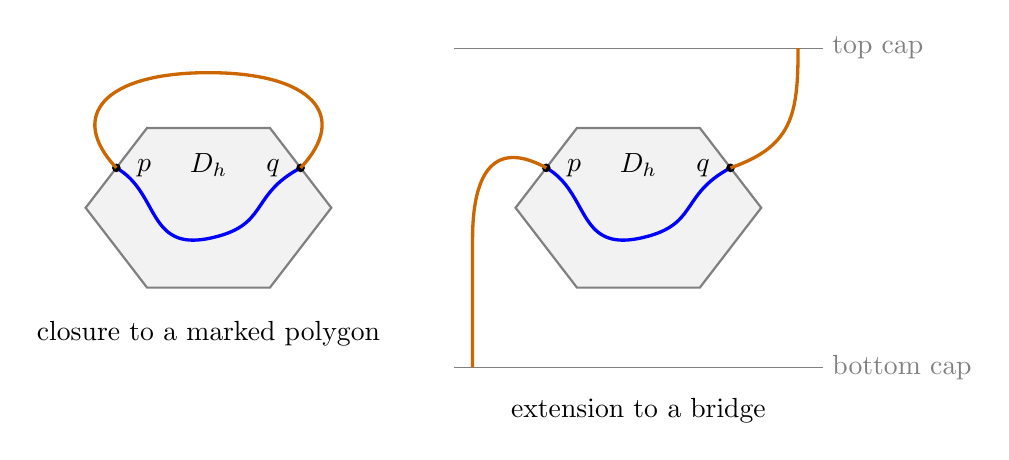
\begin{tikzpicture}[scale=.78,>=stealth]
\foreach \x in {0,7} {
  \begin{scope}[xshift=\x cm]
    \fill[gray!10] (-2,0)--(-1,-1.3)--(1,-1.3)--(2,0)--(1,1.3)--(-1,1.3)--cycle;
    \draw[gray,thick] (-2,0)--(-1,-1.3)--(1,-1.3)--(2,0)--(1,1.3)--(-1,1.3)--cycle;
    \draw[very thick,blue] (-1.5,.65) .. controls (-.8,.25) and (-1,-.7) .. (0,-.5)
      .. controls (1,-.3) and (.65,.2) .. (1.5,.65);
    \fill (-1.5,.65) circle(2pt) node[right=4pt] {$p$};
    \fill (1.5,.65) circle(2pt) node[left=4pt] {$q$};
    \node at (0,.7) {$D_h$};
  \end{scope}
}
\draw[very thick,orange!80!black] (-1.5,.65) .. controls (-2.3,1.5) and (-1.7,2.2) .. (0,2.2)
 .. controls (1.7,2.2) and (2.3,1.5) .. (1.5,.65);
\node at (0,-2.05) {closure to a marked polygon};
\begin{scope}[xshift=7cm]
 \draw[gray] (-3,2.6)--(3,2.6) node[right] {top cap};
 \draw[gray] (-3,-2.6)--(3,-2.6) node[right] {bottom cap};
 \draw[very thick,orange!80!black] (-1.5,.65) .. controls (-2.5,1.2) and (-2.7,.3) .. (-2.7,-.5)--(-2.7,-2.6);
 \draw[very thick,orange!80!black] (1.5,.65) .. controls (2.5,1) and (2.6,1.5) .. (2.6,2.6);
 \node at (0,-3.3) {extension to a bridge};
\end{scope}
\end{tikzpicture}
\caption{The two exterior sewing operations. The blue path is the chord being tested; the orange portions stay outside the convex domain. The proof realizes these schematic curves through pure-direction corridors and varies their intermediate cuts. The two boundary crossings recover the original chord for a fixed cut choice.}
\label{fig:sewing}
\end{figure}


\paragraph{Exterior connectors.}
Here are the geometric constructions and their mass bounds. For 1 close by a connector strictly in the exterior with diameter at most \(C l\), fixed endpoints \(p,q\), mass available \(\ge c l^{-5/4}\). For 2 append from \(p,q\) separate exterior paths to the two caps without touching either cap earlier, also within distance \(C R\) of the origin; together their available mass is at least \(cR^{-1/2}\exp[-C(1+\log^+(R/l))]\). In both cases for large \(l\) arrange that both exterior branches advance from their initial endpoints locally in disjoint patches of small size compared with \(l\) until reaching distance \(\rho l\) from \(D_h\), and all exterior portions between/beyond these visits stay at distance at least \(\rho l\) (sufficiently small fixed \(\rho>0\)). Even enlarged a little each patch sees only facets of a single consecutive-normal pair for outer and inner cuts used together below.

For 1, work in units \(l\), so the endpoints are separated. Take initial straight pieces along their respective outward pure normals, followed by two disjoint simple routes in the open exterior approaching a common terminal pure line from the same side in the pure perpendicular direction at two separated but close points. Around this terminal patch keep a free half-ball with radius much greater than the terminal separation (so the preceding confined arch lemma applies). The pieces other than this terminal arch can be made straight in pure directions with successive turns at most \(60^\circ\), each traveled by the point-to-line lemma with small tolerances. We give details justifying uniform finite choices in this assertion.

On scaling by \(l\) and translating, any sequence has a subsequence with distinct limit endpoints and exterior of a convex polygon, wedge or half-plane as local limit (and the indicated outward support normals among active ones). Initial rays give strictly positive distance by the corresponding supporting lines, then one can follow disjoint smooth arcs in the open exterior into an unobstructed ball for the parallel terminal lanes, approaching them on the same side. Indeed one can join the initial segments by a simple detour around the enlarged convex boundary in the connected exterior, and bend in a free middle ball to enter two parallel lanes separated by any sufficiently small distance. 

One can approximate the two arcs with end straight segments retained by polygonal arcs in pure directions: track tangent displacements on short intervals using the two adjacent pure directions spanning the tangent, inserting a short common-direction step at sector transitions, and adjusting the last intersections with the common line. Mesh sufficiently small gives separation for portions distant along the arcs, and on short portions tangent continuity gives positive projection in a common direction and hence simplicity (smooth arcs can be taken piecewise with finitely many sector transitions). Now use fixed sufficiently small apertures on the finitely many legs. End placement errors are also small by choosing tolerances small enough on all stages. Nonincident portions and successive crossing neighborhoods are separated. Along a path, adjacent pieces are disjoint by staying in the required half-planes at the transverse crossing between them; the initial piece stays in its supporting half-plane throughout. 

All choices still work along the subsequence, including the localized initial deep excursions. This gives uniformity of lengths, number of steps and apertures at this scale. For bounded \(l\), a local join at bounded cost outside suffices (exterior triangles at the two edges are connected by adjacencies around the convex flat patch or corner); no deep constraint needed.

For 2 if \(l\) is at least a fixed small multiple of \(R\), the same construction in units \(R\) suffices without terminal arch, following two disjoint paths to the two caps, terminating separately on each. Such paths exist with clearance in the intervening slab by routing in a wide annulus around the convex obstacle (in cyclic order to the outgoing lanes) before going straight to the caps. 

For smaller \(l\) the points lie on the same or adjacent facets. Start along divergent pure directions: on the same facet of normal \(m\) rotate \(m\) by \(60^\circ\) in opposite directions, heading away from one another; on adjacent facets use their two outward normals. Distances along the chosen straight rays from different ends at parameters \(x,y\ge0\) are separated by at least \(c(l+x+y)\) by projection onto the common separation tangent (bisecting the tangents for adjacent facets). Supporting normal height increases at rate at least \(1/2\). Travel to a small fixed distance of order \(R\) along each, first with a point-to-line crossing at scale \(l\), then confined pure bridges along the ray to successive heights growing by factor about 2. Tolerances a sufficiently small constant times the scales work simultaneously (error accumulation bounded geometrically); these paths are disjoint, exterior, and satisfy the initial depth condition. Continue from the macroscopically separated locations by finitely many legs at scales comparable with \(R\), as above. Uniformity here follows by the same compactness on scale \(R\) even if the rays had coincident limiting starts, since their terminal segments are already outgoing and separated in the open exterior and can be continued disjointly without meeting either ray again (route outside around the polygon and the two initial segments). The total number of legs is at most \(C(1+\log^+(R/l))\).

\paragraph{Averaging intermediate levels.}
Fix one of these corridor constructions and keep \(D_h,p,q\) fixed. In both cases, vary each intermediate transverse level uniformly over the admissible levels in its own small independent window of order the local scale, the terminal pure line for case 1 shared at both ends. Let \(\nu\) be critical weight on all exterior objects with the stated confinement and depth: a path from the labelled endpoint \(p\) to \(q\) in case 1, or an ordered pair of disjoint paths from \(p,q\) to their assigned caps in case 2. Weight counts all centers in these exterior paths. For a cut list \(\mathbf u\), let \(\mathbf1_{\mathbf u}(\eta)\) indicate that the exterior object \(\eta\) follows the prescribed corridors at those levels, and put
\[
 Y(\eta)=\mathbb E_{\mathbf u}\mathbf1_{\mathbf u}(\eta),
 \qquad P=\prod_{j=1}^k s_j^{-1/4}.
\]
Here \(s_j\) are the fixed reference scales of the \(k\) legs before any completing arch; their transverse cut separations vary within comparable windows. The indicator counts an exterior object once, since its transversal crossings recover all pieces for a fixed cut list. Concatenating the confined crossings gives
\[
 \int Y\,d\nu\ge
 \begin{cases}
 c^k l^{-5/4}P,&\text{in case 1},\\
 c^k P,&\text{in case 2},
 \end{cases}
\]
after reducing the constant \(c>0\) if necessary.

For two lists, split each branch at both choices of each varied crossing, encountered in height order in its own crossing neighborhood, yielding a difference bridge there. Indeed nonincident pieces stay out of this neighborhood, and between successive crossing stages from one end the two incident half-plane constraints put all crossings of that stage in order, with an intervening portion traveling to the next stage between its respective lines (a distance comparable to its scale). More explicitly both possible renewals in one neighborhood occur before entering the next neighborhood along the path, since the later pieces in each list avoid the former and earlier pieces avoid the latter; the crossing point for each choice is unique there and the branch locally before/after satisfies its backward/forward half-plane condition. Thus the intervening costs with incoming point prescribed are \(O(s_j^{-1/4})\) again by the upper point-to-line estimate. 

In case 1 the completing arch at the later shared level costs \(O(l^{-5/4})\) for any attained endpoints, and the shared difference gives two bridge costs of order \((1+|\mathrm{gap}|)^{-1/4}\) (the arch and the last incident pieces stay after/before the shared line, other pieces avoid this terminal patch including all confined arches). Averaging the joint costs supplies an extra \(s_j^{-1/4}\) for each varied renewal per branch at scale \(s_j\). The shared difference has power \(1/2\), so this average is still integrable. In case 2 only the two final cap levels are fixed; their endpoints remain free, and both final legs have scale comparable to \(R\). Consequently
\[
 \int Y^2\,d\nu\le
 \begin{cases}
 C^k l^{-5/4}P^2,&\text{in case 1},\\
 C^k R^{1/2}P^2,&\text{in case 2}.
 \end{cases}
\]
The factor \(R^{1/2}\) in the second line removes from the second copy of \(P\) the two factors corresponding to the fixed cap levels.

Cauchy--Schwarz now gives
\[
 \nu\{Y>0\}\ge\frac{(\int Y\,d\nu)^2}{\int Y^2\,d\nu}
 \ge
 \begin{cases}
 c_1^k l^{-5/4},&\text{in case 1},\\
 c_1^k R^{-1/2},&\text{in case 2},
 \end{cases}
\]
for a fixed \(0<c_1<1\). The number of legs is bounded in case 1. In case 2 it is at most \(C(1+\log^+(R/l))\), so \(c_1^k\ge c\min(1,(l/R)^{C_0})\) for a fixed \(C_0>0\). These are the asserted connector masses. The next average varies \(D_h\) itself, using these completed exterior objects.

\paragraph{A common target measure.}
Trim the exterior choices by fractional indicators down to precisely a common lower mass \(F\asymp l^{-5/4}\) or \(F\asymp R^{-1/2}\min(1,(l/R)^{C_0})\), respectively, pointwise for \(p,q,h,D_h\). The augmented object is a polygon injecting into the cylinder in 1 (both \(D_h\) and the augmentation near zero within a small fraction of the period length), or a full bridge in 2. For a fixed cut choice one recovers the decomposition up to bounded multiplicity since there are exactly two crossings of its boundary.

Here is the common measure used for the second moment. Let \(\Omega\) contain all six phase--slope pairs, with their product probability law, and let \(\mu\) be critical weight on target polygons through the prescribed links, or on target bridges satisfying the common deterministic event in 2. Its total mass is at most \(\mathcal K\) or \(B^*\), respectively. In a level window \(I\) of size comparable to \(\epsilon l\), define \(b_h(\Gamma,\Omega)\) to be the sum over recovered ordered decompositions of \(\Gamma\) at \(\partial D_h\) of the chord-event indicator times the exterior trimming factor. The recovery bound gives \(0\le b_h\le C\). Put
\[
 X(\Gamma,\Omega)=\mathop{\mathrm{average}}_{h\in I}
 b_h(\Gamma,\Omega).
\]
The overbar below includes both this level average and support randomness. Weight multiplication and recovery give
\begin{equation}\label{eq:sewing-first-moment}
 \int X\,d(\mu\otimes\mathbb P_\Omega)\asymp F\overline E.
\end{equation}
Both factors in \(X^2\) are tested on the same target \(\Gamma\) and the same \(\Omega\).

Choose the two levels independently and uniformly in \(I\). By symmetry it suffices to integrate over \(r<s\), with the original product measure restricted to this half-square, plus any diagonal atoms. This restriction is not renormalized: conditional on \(r\), the remaining \(s\)-measure has density, or rounded atom mass, at most \(C/l\). For \(\epsilon>0\) sufficiently small, a simultaneous event splits into the chord event for \(D_r\), two exterior bridges crossing the band to \(\partial D_s\), and then the augmentation from there; keep only the latter trimming factor. Boundary crossings are unique on the separate branches, localized by the depth condition because the boundary moves by at most \(C\epsilon l+O(1)\). For bounded \(s-r\), or bounded \(l\), the indicator at \(r\) alone suffices. We will bound the averaged cost \(\Xi\) of the two band bridges uniformly conditional on the inner level and phases. This gives
\begin{equation}\label{eq:sewing-second-moment}
 \int X^2\,d(\mu\otimes\mathbb P_\Omega)
 \le CF\overline E\,\Xi.
\end{equation}

\paragraph{The two band bridges.}
Put \(g=s-r\). We bound the bridges for large \(g\) as follows. Fix for each bridge the possible target normal in the local facet pair. Drop all other outer cuts, keeping the entire inner elbow in a local patch with two lateral pure trims transversal to both tangent directions containing the bridge portions; the domain is a polygonal strip between this outward cut line and the flat or elbow piece of \(D_r\). The inner obstacle here keeps just the two corresponding consecutive constraints (or just one for a common flat region), extended throughout the strip patch; this agrees locally on the required bridge portions. The target outward cut line is thus disjoint from it by the positive gap. Trims may for instance bound projection on the common tangent bisector for a consecutive pair (a pure normal direction), wide enough to enclose the localized portions and leave clearance at the source, and can be fixed independently of the dropped outer facets. 

There is a positive contour (after a possible rotation) from the inner source. Indeed closing a chord along the boundary gives \(W\) equal to lifted outward-normal change minus \(\pi\) going round the counterclockwise perimeter from source to exit. There is only one possible reflex corner on the inner elbow, with outward normal decreasing by \(\pi/3\), and its two outward normals and the outward normals on trim sides and target line are in cyclic order except for this one corner (the trims use a pure direction strictly between opposing boundary sectors). Thus from a given inner source at most one sign of excess beyond \([-\pi,\pi]\) occurs, and by at most \(\pi/3\); rotating gives real coefficients bounded below positively since \(\beta=3/8\). Convexity is not needed for the contour identity on this simply connected domain. 

Cut down by a centered triangle at scale a small multiple of \(\min(g,t_i)\), where the inner source is on a flat side. By contour subtraction and the escape upper estimate its bridge cost is \(O((1+\min(g,t_i))^{-1/4})\). This also holds by the full positive contour when the minimum is bounded. 

For the corner gain, put \(t=\min_i t_i\). Both tests in \(X^2\) use the same dyadic endpoint bins: the two inner bin sizes are at least \(t\), and one outer bin has size of order \(t\). Sum over the finitely many choices of that outer endpoint and of the facet it reaches. For each choice, condition on the six phases at \(r\), making the inner chord event measurable, and on the support position of the selected target facet at \(s\). Figure~\ref{fig:sewing-band} shows the adjacent outer facet whose support has not been revealed.
\begin{figure}[htbp]
\centering
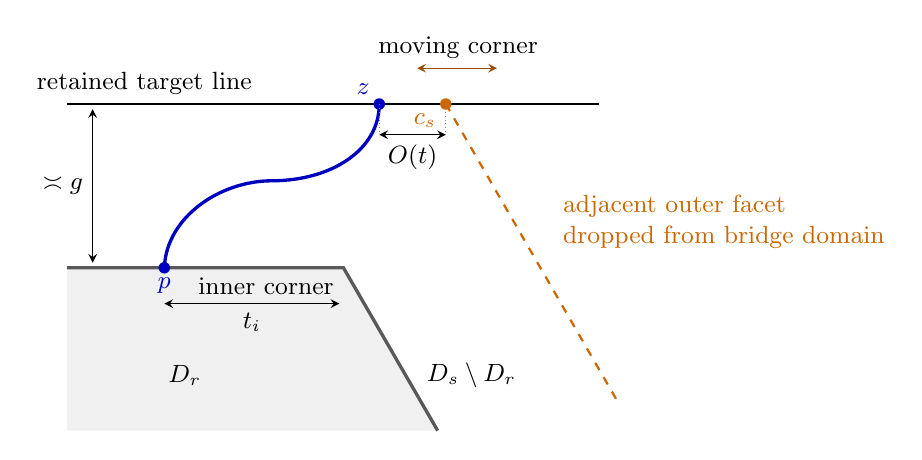
\begin{tikzpicture}[scale=1.3,>=stealth,font=\small]
 \fill[gray!12] (-2.7,0)--(0,0)--(.92,-1.59)--(-2.7,-1.59)--cycle;
 \draw[gray!70!black,very thick] (-2.7,0)--(0,0)--(.92,-1.59);
 \node at (-1.55,-1.05) {$D_r$};
 \node at (1.25,-1.05) {$D_s\setminus D_r$};
 \node[below left] at (0,0) {inner corner};
 \draw[thick] (-2.7,1.6)--(2.5,1.6);
 \node[above left] at (-.8,1.6) {retained target line};
 \draw[orange!80!black,thick,dashed] (1,1.6)--(2.7,-1.344);
 \draw[orange!60!black,<->] (.72,1.95)--(1.5,1.95);
 \node[above] at (1.12,1.95) {moving corner};
 \node[orange!80!black,align=left,anchor=west] at (2.05,.45)
   {adjacent outer facet\\dropped from bridge domain};
 \fill[orange!80!black] (1,1.6) circle(1.6pt) node[below left] {$c_s$};
 \draw[blue!75!black,very thick] (-1.75,0)
   .. controls (-1.73,.5) and (-1.2,.85) .. (-.7,.85)
   .. controls (-.12,.85) and (.35,1.15) .. (.35,1.6);
 \fill[blue!75!black] (-1.75,0) circle(1.6pt) node[below] {$p$};
 \fill[blue!75!black] (.35,1.6) circle(1.6pt) node[above left] {$z$};
 \draw[<->] (.35,1.3)--(1,1.3) node[midway,below] {$O(t)$};
 \draw[gray,densely dotted] (.35,1.6)--(.35,1.3);
 \draw[gray,densely dotted] (1,1.6)--(1,1.3);
 \draw[<->] (-1.75,-.35)--(-.04,-.35) node[midway,below] {$t_i$};
 \draw[<->] (-2.45,.05)--(-2.45,1.55) node[midway,left] {$\asymp g$};
\end{tikzpicture}
\caption{The selected band bridge from an inner port $p$ to an outer port $z$, with $g=s-r$. The inner elbow is retained when bounding the bridge, while the dashed adjacent outer facet is dropped. After fixing the target support, the adjacent support is still independent and has conditional density, or row-atom bound, $O(1/g)$. Its intersection $c_s$ with the target therefore falls within $O(t)$ of a fixed $z$ with probability at most $C\min(1,t/(1+g))$, including row rounding. The diagram is schematic; the second band bridge is bounded uniformly without revealing this support.}
\label{fig:sewing-band}
\end{figure}


For any attained outer endpoints and support choices, integrate the outer completion to its constant trimmed mass \(F\). Bound the other band bridge uniformly after dropping its extra avoidance constraints. This bound does not require revealing the adjacent outer support, even if the other bridge ends on that facet.

The adjacent outer facet defining the selected endpoint's corner is therefore still unconditioned. Its position is independent of the selected target support, conditional on the inner phases, and has density \(O(1/g)\). This remains true because \(V_i+A_i r/R\) modulo one is uniform and independent of \(A_i\). Since that adjacent facet was dropped from the selected bridge domain, each possible end has probability at most \(C\min(1,t/(1+g))\) of being within \(O(t)\) of its corner, also after lattice rounding. We average this corner event instead of conditioning on it. Both inner endpoint bin sizes are at least \(t\), so the product of the two bridge bounds is uniform in the support parameter still being averaged. The resulting joint cost is therefore
\[
 C(1+\min(g,t))^{-1/2}\min\{1,t/(1+g)\}
 \le C(1+g)^{-1/2}.
\]

The conditional gap estimate gives \(\Xi\le Cl^{-1/2}\) on each window. Applying Cauchy--Schwarz to \eqref{eq:sewing-first-moment}--\eqref{eq:sewing-second-moment} yields
\[
 \overline E\le C\mathcal K\,\Xi/F,
 \qquad B^*\ge cF\overline E/\Xi,
\]
respectively. Substitution of \(F\) and \(\Xi\) proves both sewing assertions. Averaging these inequalities recombines the windows.
\end{proof}

\subsection{Corner gains and the marked-pair sum}\label{sec:corner-sum}

The previous estimate is sufficient for one endpoint bin. To sum all bins with a bounded constant, we retain the gain when an endpoint lies close to a corner. Write $t=\min(t_1,t_2)$, with $1\le t\le l$. The two estimates before averaging the cut gap $g$ give the combined cost
\[
 C(1+\min(g,t))^{-1/2}\min\{1,t/(1+g)\}.
\]
For each fixed inner level $r$, the unnormalized gap law on the half-square $r<s$ has density at most $C/l$ over an interval of length $O(l)$, with the analogous bound for its rounded discrete law. This uniformity allows the estimate to be integrated against the possibly nonconstant mass $E_r$. Splitting at $g=t$ shows that its average is at most
\[
 \frac C l\left(\int_0^t(1+g)^{-1/2}\,dg
 +t(1+t)^{-1/2}\int_t^{Cl}\frac{dg}{1+g}\right)
 \le C_\eta l^{-1/2}(t/l)^\eta
\]
for any fixed $0<\eta<1/2$. The bounded-gap atoms satisfy the same estimate after increasing $C_\eta$.

Keeping this gain in the first sewing argument gives
\begin{equation}\label{eq:sewing-corner-gain}
 \overline E\le C_\eta l^{3/4}(t/l)^\eta\mathcal K.
\end{equation}
Indeed the first moment in the target polygon measure is at least $cF\overline E$, while the second is at most
$CF\overline E\,l^{-1/2}(t/l)^\eta$; use $F\asymp l^{-5/4}$. For each smaller corner bin $t$, the larger one has only $O(1+\log(l/t))$ possible dyadic values. Thus their total contribution is bounded by
\[
 C_\eta\sum_{j\ge0}(1+j)2^{-j\eta}<\infty.
\]
The same summation shows that bins with $t/l\le\delta$ have total coefficient tending to zero as $\delta\downarrow0$.

Let $\ell_h$ denote the length of a chord in $D_h$, and retain chords of diameter at least $R/3$. Their mass is at most $CR^{3/4}$. Their first-length mass is at least $cR^{25/12}$: every path through a sufficiently central link is macroscopic, and Proposition~\ref{prop:occupancy} with Theorem~\ref{thm:nesting} supplies mass at least $cR^{1/12}$ at each of $cR^2$ such links. The upper first-length mass over all chords is $CR^{25/12}$ by the same identity.

To estimate the second moment, first omit the initial and terminal visited centers. The ordered pairs involving these at most two centers number $O(\ell_h)$, so their integrated contribution is absorbed by the first-length bound. At each remaining center, record the directions of the two tiling edges crossed by its incident path links. Divide these centers into finitely many classes according to triangle type, lattice translation modulo two, and that pair of tiling-edge directions. The square of the total number of remaining centers is bounded by a fixed multiple of the sum of the squares of the class counts. Within a class, pairs with axial or zero displacement contribute at most $CR\ell_h$ for each chord: a bounded domain of diameter $CR$ has only $CR$ positions on the finitely many axial lines through a given center. Their integrated contribution is therefore at most $CR^{37/12}$.

For a remaining ordered pair, choose the two lattice axes spanning the strict sector containing its displacement. At least one of the two recorded tiling-edge directions is one of those axes. Since the two centers have the same triangle type, the corresponding crossed edges are translates and supply identical axial marks used by internal links of the chord. Their displacement has even coordinates in the chosen lattice basis, by the translation class modulo two. Hence $d=P_1+P_2$ is even, as required in Theorem~\ref{thm:two-marks}. Choose an integer period multiple $kP$ with length comparable to a sufficiently large constant times $R$, so the sewn polygon projects injectively. Then $N\asymp R$ and
\[
 \mathcal K\le C R^{-4/3}(R/d)^{15/8}.
\]
There are $O(R^2)$ choices of the first center and $O(d)$ displacements with $P_1+P_2=d$. Consequently
\begin{equation}\label{eq:marked-pair-sum}
 \sum_{\text{eligible pairs}}\mathcal K
 \le CR^2R^{-4/3}R^{15/8}\sum_{1\le d\le CR}d^{1-15/8}
 \le CR^{8/3}.
\end{equation}
Apply \eqref{eq:sewing-corner-gain} to each pair event. The corner bins sum with bounded total coefficient, and the separation factors $l^{3/4}$ sum geometrically up to $CR$. We obtain
\begin{equation}\label{eq:chord-second-moment}
 \overline{\sum_{\gamma\text{ macroscopic in }D_h}
       \ell(\gamma)^2w(\gamma)}\le CR^{41/12}.
\end{equation}
The contribution from bins $l\le\delta R$ has upper bound
$C\delta^{3/4}R^{41/12}+CR^{37/12}$. On the remaining separations, bins with $t\le\delta'R$ likewise have arbitrarily small relative coefficient when $\delta'$ is sufficiently small. These are estimates for actual endpoint restrictions on the chords, not an assumption that endpoints avoid corners.

\subsection{A positive fraction of long bridges}

We now prove \eqref{eq:bridge-long-fraction}. Write $M_1$ for the averaged first-length mass of the macroscopic chords. We have $M_1\ge c_1R^{25/12}$. By Cauchy--Schwarz, a class with second moment at most $\varepsilon R^{41/12}$ contributes at most
\[
 (CR^{3/4}\cdot\varepsilon R^{41/12})^{1/2}
 =C\sqrt\varepsilon\,R^{25/12}
\]
to $M_1$. Choose $\delta>0$ and then $\delta'>0$ so that removal of close endpoints and small corner bins loses less than one quarter of $M_1$. Chords shorter than $aR^{4/3}$ contribute at most $CaR^{25/12}$, which is less than another quarter if $a>0$ is fixed sufficiently small.

The retained chords therefore have averaged first-length mass at least $c_2R^{25/12}$. Their endpoint separation and corner distances are all bounded below by fixed multiples of $R$, so they occupy only a bounded number of bins. In at least one bin the first-length mass has the same lower order. Applying Cauchy--Schwarz to that bin and \eqref{eq:chord-second-moment} gives its averaged ordinary mass at least
\[
 c\frac{R^{50/12}}{R^{41/12}}=cR^{3/4}.
\]
The second sewing estimate extends these chords to bridges between any prescribed pair of horizontal caps whose distances above and below the origin lie in $[AR,2AR]$, for a fixed sufficiently large $A$. Since $l\asymp R$, that estimate gives total bridge mass at least $cR^{3/4}$ when the bottom start is free over the permitted interval of $O(R)$ ports. Every output bridge contains the retained chord, and hence has length at least $aR^{4/3}$.

Translation invariance makes the unrestricted mass from each bottom port equal. Removing the confinement and dividing by the number of permitted starting ports yields
\[
 B_h\{\ell\ge aR^{4/3}\}\ge cR^{-1/4}
\]
for every admissible cap separation $h d_0\in[2AR,4AR]$. For an arbitrary sufficiently large integer $h$, choose $R$ proportional to $h$ so the selected caps lie in these ranges; admissible rounding changes only fixed constants. This proves \eqref{eq:bridge-long-fraction} at every sufficiently large height.

\subsection{The strip first moment and completion of the proof}

It remains to prove the first-length upper bound. In the infinite strip, summing occurrences of internal links over bridges from one fixed bottom port is the same as summing the occurrence mass with free bottom port over link representatives modulo translations along the strip. There are $O(h)$ such representatives. Proposition~\ref{prop:occupancy}, first in finite convex truncations and then by monotone exhaustion, bounds the occurrence mass at each link by the positive enclosing-polygon partitions at its adjacent lattice points.

These partitions are at most $Ch^{1/12}$ even though the strip is infinite. To see this, take a pure lattice period vector tilted relative to the strip's horizontal tangent, of sufficiently large even length comparable to $h$, with transverse projection greater than $2h d_0$. The strip and its translate by half this period embed disjointly in the resulting cylinder. The disk enclosed by each polygon stays inside its convex strip, so it cannot contain the mark in the translated strip. Thus two independent systems enclosing corresponding points inject into a system separating the antipodal marks. The bounded-factor cylinder estimate in Section~\ref{sec:uniform-nesting} is at most $Ch^{1/6}$, so the square of the strip partition is at most that quantity.

Summing over the $O(h)$ link representatives gives
\[
 \sum_{\gamma\in\mathcal B_h}(\ell(\gamma)-1)w(\gamma)
 \le Ch^{13/12}.
\]
The missing one center per bridge adds only $B_h\le Ch^{-1/4}$. This proves \eqref{eq:bridge-first-moment}. The strip mass \eqref{eq:bridge-mass} was proved in Sections~\ref{c6:strip-transfer}--\ref{c6:strip-asymptotics}, and Proposition~\ref{prop:crossings} gives \eqref{eq:bridge-diameter}. Theorem~\ref{thm:finite-bridges} is complete.
